\documentclass{article} %this is an article
\usepackage[lmargin=.75in,rmargin=.75in,tmargin=1.in,bmargin=1in]{geometry} % setting margins
%\usepackage{tree-dvips}
\usepackage{tikz}  %makes crazy graphs
\usepackage{enumitem}
% \usetikzlibrary{snakes}
%\usepackage[flushleft]{threeparttable} %% makes notes for tables that wraps around width of table
%\usepackage{chronology}
\usepackage[round]{natbib}  %% beatiful bibliography
%\usepackage{wrapfig}
%\usepackage{longtable} %%multipage table
%\usepackage{qtree}
\usepackage{verbatim} %all kinds of shit
\usepackage{graphicx} %beautiful figures
%\usepackage{graphics}
%\usepackage{color}
%\usepackage{caption}
\usepackage{subcaption} %subcaption on the the subfigures
%\usepackage{multirow}
%\usepackage{sidecap}
%\usepackage{epstopdf}
\usepackage{amssymb} %beautiful math
\usepackage{amsmath,amssymb,amsfonts,amsthm,array} %beautiful math
\usepackage{amsthm}  %beautiful math
\usepackage{pgfplots}  %Normal distribution figure
\usepackage[colorlinks=true,linkcolor=red, citecolor=red]{hyperref} %sets my preferences for cross reference



\begin{document}
\begin{center}
  \textbf{Joao Rodrigues} \\
  \textbf{Economics 8185 - Computational Methods} \\
  \textbf{Homework 1} \\
  \textbf{Economics Department}
\end{center}
%%%
In this assignment, I replicated the results from the Business Cycle Accounting paper by Chrari, Kehoe, and Mcgrattan. I did so for their benchmark economy. By replicating their results, I derived the implied wedges that come from applying maximum likelihood estimation to the process that governs the exogenous shocks to the economy given that the economy evolves according to the linearized policy functions.
\\
\\
I followed the appendix for the paper in order to solve the model. Hence my first exercise was to replicate the results for the United States presented in the paper. I didn't derive the parameters for the linearized variables by hand as it was done in the appendix. Rather I used numerical differentiation to both linearize the equality constraints, and to derive a gradient for the euler equation to solve the second order difference equation needed for the policy function.   
\\
\\
In order to maximize the likelihood function I used the adaptive Nelder-Mead algorithm which is the default version of Nelder mead in Julia as opposed to the fixed parameter version of the original paper. I used the same strategy imposed by Ellen in her code where I maximized the functions several times, adding disturbances each time, storing the results in an array and taking the maximum. This was key in order to solve the model for the United States, although for Australia, the algorithm went to the maximum pretty fast. This portion of the code os muted as it takes a long time but it's there if you want to test the code. The result is ausestJP.txt for Australia and usest.txt for the United States that is saved in the homework folder.
\\
\\
In order to apply BCA to Australia I used the data collected by Brinca - who applied BCA to OECD countries - which contains macro data for OECD countries. I then followed his appendix to clean the data in order to render it usable for BCA. 
\section*{Implied wedges}
%
For the United States, the picture attached here is a replication of figure 5 in the paper but adding the government wedge to the figure as well. It covers the period from the first quarter of 1979 to the last quarter of 1985 as a way of analyzing the recession of 1982. For the United States it's clear that productivity and labor wedges are more significant in driving the decline in output observed. 
%
\begin{figure}[h!]
  \centering
  \begin{subfigure}[b]{0.45\textwidth}
    %\centering
  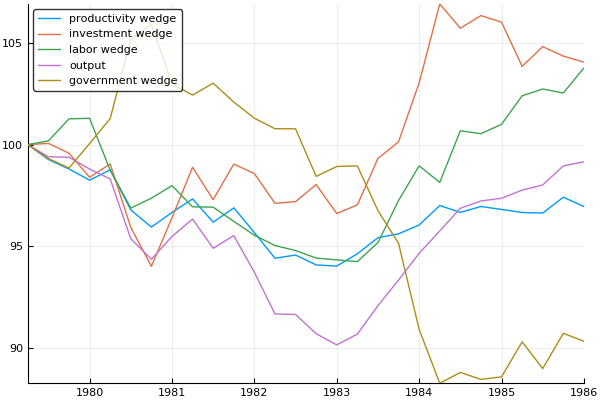
\includegraphics[width=\textwidth]{../USA/us_wedges.png}
  \caption{Implied wedges for the United States}
\end{subfigure}
\begin{subfigure}[b]{0.45\textwidth}
  %\centering
  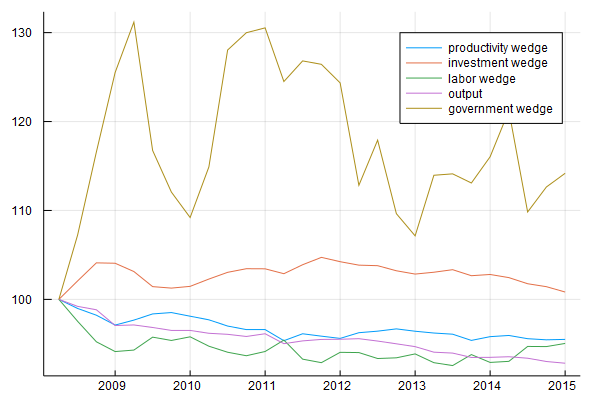
\includegraphics[width=\textwidth]{../AUS/wedges.png}
  \caption{Implied wedges for Australia}  
  \end{subfigure}
\end{figure}
%
For Australia, the period covered is from the first quarter of 2008 to the last quarter of 2014. As far as Australia, we can see that despite wild swings in the government wedges, output declines steadly along side productivity and labor wedges as it happened in the united States. In fact, the investment wedge is above trend througout the entire recessionary period. Potentially, the recession drove down investment goods prices and while investment took place, it did not pull Australia out of the recession.  

\section*{Files}
The main folder cointains the julia file BCAq.jl which defines all the functions needed to solve the model including the likelihood function. Then there are several folders:
\begin{itemize}
\item latex
  contains this file and notes.pdf is a file with some but not all of my notes on this exercise. 
\item AUS
  BCA\_AUS.jl along with ausdata.txt generated by the matlab files in matlab\_datawork
\item USA
  BCA\_USA.jl along with usdata.txt generated by the matlab files in matlab\_datawork
\item matlab\_datawork
  AUSdatawork.m and calgz.m and running AUSdatawork generates the Australian data and puts it in the AUS folder. The dada needed to generate ausdata.txt in also contained in this folder.  
  \end{itemize}

%\bibliographystyle{plainnat}
%\bibliography{hw1.bib}
\end{document}
